\section{Projet de recherche}
\subsection{Dummy}

\begin{frame}{Cohérence et thermalisation dans les systèmes en interaction}
\textbf{Objectifs} : ingénierie de systèmes robustement cohérents, compréhension du couplage à l'environnement et thermalisation.

\textbf{Contexte grenoblois} : manipulation de qubits (institut Néel, CEA), théorie des systèmes quantiques (LPMMC, institut Néel, CEA, LIG).

\begin{columns}
	\begin{column}{0.5\textwidth}
		\centering
		\includegraphics[height=3cm]{img/2_projet_recherche/Godfrin_YbQudit_closeup}
	\end{column}
	\begin{column}{0.6\textwidth}
		\centering
		\includegraphics[height=3cm]{img/2_projet_recherche/Godfrin_coherence_time}
	\end{column}
\end{columns}
{

\centering
Qudit couplé à une boîte quantique {\footnotesize[Godfrin \emph{et al} 19]}

}

\textbf{Méthodes} : numériques (diagonalisation exacte, DMRG), analytiques (circuits quantiques).
\end{frame}

\begin{frame}{Cohérence robuste : cicatrices quantiques}
\begin{columns}
	\begin{column}{0.5\textwidth}
		\centering
		\includegraphics[height=3cm]{img/2_projet_recherche/scars_spin_polarization}
		
		États non-ergodiques dans une mer chaotique
		
		\footnotesize{[Turner \emph{et al} 18]}
	\end{column}
	\begin{column}{0.5\textwidth}
		\centering
		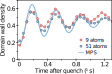
\includegraphics[height=3cm]{img/2_projet_recherche/scars_DW_density}
		
		Expérience : blocage de Rydberg
		
		\footnotesize{[Bernien \emph{et al} 17]}
	\end{column}
\end{columns}
\begin{block}{\textbf{Projet} [Anna Minguzzi, Robert Whitney]}
	\begin{itemize}
		\item Conditions d'existence ?
		\item Couplage à l'environnement ?
	\end{itemize}
\end{block}
\end{frame}

\begin{frame}{Circuits quantiques}
\begin{enumerate}
	\item Structure simple $\to$ description \textbf{exacte}
	\item Hydrodynamique (grands $t$ et $x$) $\to$ description \textbf{universelle}
\end{enumerate}
\begin{columns}
	\begin{column}{0.5\textwidth}
		\centering
		\includegraphics[height=3cm]{img/2_projet_recherche/circuit}
				
		\footnotesize{[Chan, De Luca, Chalker 18]}
	\end{column}
	\begin{column}{0.6\textwidth}
		\begin{block}{\textbf{Projet} \footnotesize{[L.\ Canet, V.\ Rossetto, C.\ Branciard, P.\ Arrighi]}}
			\begin{itemize}
				\item Systèmes critiques ?
				\item Désordre ? 2D ?
				\item Dynamique de l'information et efficacité des algorithmes quantiques ?
			\end{itemize}
		\end{block}
		\begin{block}{\textbf{Expertise numérique}}
			Diagonalisation exacte innovante
		\end{block}
	\end{column}
\end{columns}
\end{frame}
